\documentclass[fleqn, a4paper, 11pt, oneside]{amsart}
%\usepackage[top = 2cm, bottom = 1cm, left = 1cm, right = 1cm]{geometry}
\usepackage{exsheets, tasks}
\usepackage{amsmath, amssymb, amsthm} %standard AMS packages
\usepackage{marginnote} %marginnotes
\usepackage{gensymb} %miscellaneous symbols
\usepackage{commath} %differential symbols
\usepackage{xcolor} %colours
\usepackage{cancel} %cancelling terms
\usepackage{siunitx} %formatting units
\usepackage{tikz, pgfplots} %diagrams
\usetikzlibrary{calc, hobby, patterns, intersections}
\usepackage{graphicx} %inserting graphics
\usepackage{hyperref} %hyperlinks
\usepackage{datetime} %date and time
\usepackage{ulem} %underline for \emph{}
\usepackage{xfrac} %inline fractions
\usepackage{enumerate,enumitem} %numbered lists
\usepackage{float} %inserting floats
\usepackage{circuitikz} %circuit diagrams

\newcommand\numberthis{\addtocounter{equation}{1}\tag{\theequation}} %adds numbers to specific equations in non-numbered list of equations

\newcommand{\AxisRotator}[1][rotate=0]{
	\tikz [x=0.25cm,y=0.60cm,line width=.2ex,-stealth,#1] \draw (0,0) arc (-150:150:1 and 1);%
} %rotation symbols on axes

\theoremstyle{definition}
\newtheorem{example}{Example}
\newtheorem{definition}{Definition}

\theoremstyle{theorem}
\newtheorem{theorem}{Theorem}

\newcommand{\curl}{\mathrm{curl\,}}

\makeatletter
\@addtoreset{section}{part} %resets section numbers in new part
\makeatother

\renewcommand{\thesubsection}{(\arabic{subsection})}
\renewcommand{\thesection}{(\arabic{section})}

%section headings on left
\makeatletter
\def\specialsection{\@startsection{section}{1}%
	\z@{\linespacing\@plus\linespacing}{.5\linespacing}%
	%  {\normalfont\centering}}% DELETED
	{\normalfont}}% NEW
\def\section{\@startsection{section}{1}%
	\z@{.7\linespacing\@plus\linespacing}{.5\linespacing}%
	%  {\normalfont\scshape\centering}}% DELETED
	{\normalfont\scshape}}% NEW
\makeatother

%forces newline after subsection
\makeatletter
\def\subsection{\@startsection{subsection}{3}%
	\z@{.5\linespacing\@plus.7\linespacing}{.1\linespacing}%
	{\normalfont\itshape}}
\makeatother

\settasks{counter-format = tsk[1].}

\SetupExSheets{solution/print = true}

%opening
\title{Physics 2 : Assignment 7}
\author
{
	Aakash Jog\\
	ID : 989323563
}
\date{\formatdate{13}{5}{2015}}

\begin{document}

\maketitle
%\setlength{\mathindent}{0pt}

\begin{question}
	A common textbook question asks you to calculate the resistivity of a cone shaped object of resistivity $\rho$, with length $L$, radius $a$ at one end and radius $b$ at the other end, as shown.
	The two ends are flat and are taken to be equipotential.
	The suggested method is to slice it into thin circular discs of width $\dif z$, calculate each disk's resistivity and integrate to get the total.
	\begin{figure}[H]
		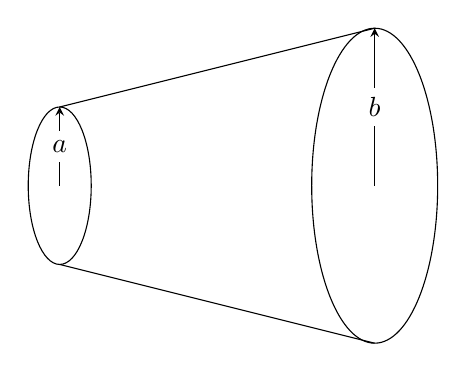
\begin{tikzpicture}
			\def\a{1};
			\def\b{2};
			\def\r{1.5};
			\def\dr{0.1};
			\def\L{4};

			\draw (0,0) circle [x radius = 0.4*\a, y radius = \a];
			\draw (\L,0) circle [x radius = 0.4*\b, y radius = \b];

			\draw
				(0,\a) -- (\L,\b)
				(0,-\a) -- (\L,-\b);

			\begin{scope}[-stealth]
				\draw (0,0) -- ++(0,\a) node [midway, fill = white] {$a$};
				\draw (\L,0) -- ++(0,\b) node [midway, fill = white] {$b$};
			\end{scope}
		\end{tikzpicture}
	\end{figure}
	\begin{enumerate}
		\item Calculate the resistance, $R$, in this way.
		\item Try to explain why this method is fundamentally flawed.
		\item
			Suppose that the ends are, instead, spherical surfaces centered at the apex of the cone.
			Calculate the resistance $R$ in this case.
			Let $L$ be the distance between the centers of the circular perimeter of the end cups.
	\end{enumerate}
\end{question}

\begin{solution}
	\begin{enumerate}[leftmargin = *]
		\item
			\begin{align*}
				\dif R       & = \rho \frac{\dif z}{\pi r^2}                                              \\
                                             & = \rho \frac{\dif z}{\pi \left( \left( \frac{b - a}{L} \right)z \right)^2} \\
                                             & = \rho \frac{\dif z}{\pi \left( \frac{(b - a)^2 z^2}{L^2} \right)}         \\
				\therefore R & = \frac{L^2}{(b - a)^2}\int\limits_{0}^{L} \frac{\dif z}{z^2}              \\
                                             & = \frac{\rho L}{\pi a b}
			\end{align*}
		\item
			The current flowing in the elemental disk is not perpendicular to the disk itself.
			Therefore, the length of the elemental resistor with respect to the current is not $\dif z$ but $\frac{\dif z}{\cos \theta}$ where $\theta \in [0, \theta_0]$, where $\theta_0$ is the apex angle of the cone.
	\end{enumerate}
\end{solution}

\begin{question}
	Two concentric metal spherical shells, of radius $a$ and $b$, respectively, are separated by weakly conducting material of conductivity $\sigma$.
	\begin{enumerate}
		\item If they are held at potential difference $V$, calculate the current flow from one to the other.
		\item What is the resistance between the shells?
		\item
			Notice that if $b >> a$ than the outer radius $b$ becomes irrelevant.
			How do you account for that?
			Use this to calculate the current flowing between two metal spheres of radius $a$, immersed deep in the sea and held very far apart, if the potential difference between them is $V$.
	\end{enumerate}
\end{question}

\begin{solution}
	\begin{enumerate}[leftmargin = *]
		\item
			\begin{align*}
				I & = \int j \dif A        \\
                                  & = \int \sigma E \dif A \\
				\intertext{Consider a spherical Gaussian surface with radius $b$. Therefore, by Gauss' Law, $E = \frac{Q}{\varepsilon_0}$. Therefore,}
				I & = \sigma \frac{Q}{\varepsilon_0}
			\end{align*}
			\begin{align*}
				V            & = -\int\limits_{b}^{a} E \dif r                                          \\
                                             & = \int\limits_{a}^{b} \frac{Q}{4 \pi \varepsilon_0 r^2} \dif r           \\
                                             & = \frac{Q}{4 \pi \varepsilon_0} \left( \frac{1}{a} - \frac{1}{b} \right) \\
				\therefore Q & = \frac{4 \pi \varepsilon_0 V}{\frac{1}{a} - \frac{1}{b}}
			\end{align*}
			Therefore,
			\begin{align*}
				I & = \sigma \frac{4 \pi \varepsilon_0 V}{\frac{1}{a} - \frac{1}{b}}
			\end{align*}
		\item
			\begin{align*}
				R            & = \frac{V}{I}                                                \\
				\therefore R & = \frac{V}{\frac{4 \sigma \pi V}{\frac{1}{a} - \frac{1}{b}}} \\
                                             & = \frac{\frac{1}{a} - \frac{1}{b}}{4 \sigma \pi}
			\end{align*}
		\item
			If $b >> a$,
			\begin{align*}
				R & = \frac{\frac{1}{a} - \frac{1}{b}}{4 \sigma \pi \varepsilon_0} \\
                                  & = \frac{1}{4 a \sigma \pi \varepsilon_0}
			\end{align*}
			If two metal spheres of radius $a$ are immersed in the sea and held very far apart, the equivalent resistance that due to the two sphered in series.
			Therefore the net resistance is $2 R$, where $R$ is the resistance due to one metal sphere.\\
			Therefore,
			\begin{align*}
				I & = \frac{V}{2 R}                      \\
                                  & = \frac{V}{\frac{2}{4 a \sigma \pi}} \\
                                  & = 2 a V \sigma \pi
			\end{align*}
	\end{enumerate}
\end{solution}

\end{document}
